\documentclass{beamer}

\mode<presentation>
{
  \usetheme{Warsaw}
  % or ...

  \setbeamercovered{transparent}
  % or whatever (possibly just delete it)
}

\usepackage{standalone}
\usepackage{tikz}
\usepackage[english]{babel}
% or whatever

\usepackage[utf8]{inputenc}
% or whatever
\usepackage[outdir=./]{epstopdf}
\usepackage{times}
\usepackage[T1]{fontenc}
% Or whatever. Note that the encoding and the font should match. If T1
% does not look nice, try deleting the line with the fontenc.


\title[Data Sharing and Citations] % (optional, use only with long paper titles)
{Combined Regression Results}

\subtitle
{Causal Evidence} % (optional)

\author[Christensen, Dafoe, Miguel] % (optional, use only with lots of authors)
{Garret Christensen\inst{1} \and Allan Dafoe\inst{2} \and Edward Miguel\inst{3}}
% - Use the \inst{?} command only if the authors have different
%   affiliation.

\institute[Universities of Somewhere and Elsewhere] % (optional, but mostly needed)
{
  \inst{1}%
  Berkeley Institute for Data Science, UC Berkeley
  \and
  \inst{2}%
  Department of Political Science, Yale University
  \and
  \inst{3}%
  Department of Economics, UC Berkeley}
% - Use the \inst command only if there are several affiliations.
% - Keep it simple, no one is interested in your street address.

\date[Short Occasion] % (optional)
{April 2018}

\subject{Talks}
% This is only inserted into the PDF information catalog. Can be left
% out. 



% If you have a file called "university-logo-filename.xxx", where xxx
% is a graphic format that can be processed by latex or pdflatex,
% resp., then you can add a logo as follows:

% \pgfdeclareimage[height=0.5cm]{university-logo}{university-logo-filename}
% \logo{\pgfuseimage{university-logo}}



% Delete this, if you do not want the table of contents to pop up at
% the beginning of each subsection:
%\AtBeginSubsection[]
%{
%  \begin{frame}<beamer>{Outline}
%    \tableofcontents[currentsection,currentsubsection]
%  \end{frame}
%}


% If you wish to uncover everything in a step-wise fashion, uncomment
% the following command: 

%\beamerdefaultoverlayspecification{<+->}


\begin{document}
{ % all template changes are local to this group.
    \setbeamertemplate{navigation symbols}{}
    \begin{frame}[plain]
        \begin{tikzpicture}[remember picture,overlay]
            \node[at=(current page.center)] {
                \href{https://www.bitss.org/}{
\includegraphics[width=\paperwidth]{../images/BITSSlogo.png}}
            };
        \end{tikzpicture}
     \end{frame}
}

\begin{frame}
  \titlepage
  \begin{center}
  \begin{large}
  PRELIMINARY--Please do not cite.
  \end{large}
  \end{center}
\end{frame}

\begin{frame}
Thanks to David Birke, Mu Yang Shin, Don Sun, Manana Hakobyan, Terri Cruz, Maxim Guzman, Baiyue Cao, Evey Huang, Rachel Kim, Ravina Pattni, Kevin Khuu, Neil Tagare, Simon Zhu, Jacqueline Wood, Kai Ong, Isabel Zhou
\end{frame}

%\begin{frame}{Outline}
 % \tableofcontents
  %\begin{center}
 % Slides available at: \url{http://www.github.com/bitss/citations}
  %\begin{large}
 % PRELIMINARY--Please do not cite.
  %\end{large}
 % \end{center}
  % You might wish to add the option [pausesections]
%\end{frame}


% Since this a solution template for a generic talk, very little can
% be said about how it should be structured. However, the talk length
% of between 15min and 45min and the theme suggest that you stick to
% the following rules:  

% - Exactly two or three sections (other than the summary).
% - At *most* three subsections per section.
% - Talk about 30s to 2min per frame. So there should be between about
%   15 and 30 frames, all told.
	
%\section{Introduction}

%\begin{frame}{Data Sharing Incentives}{}
%  % - A title should summarize the slide in an understandable fashion
%  %   for anyone how does not follow everything on the slide itself.
%
%  \begin{itemize}
%  \item
%    Shared data is a public good. (See Newton 1675)
%  \item
%    Public goods are often undersupplied.
%  \item 
%  	 Is there private incentive?
%  	 \begin{itemize}
%  	 \item Promotion \& tenure
%  	 \item Citations
%  	 \end{itemize} 
%  \end{itemize}
%\end{frame}
%
%\begin{frame}{Citations}
%\begin{itemize}
%\item Signal of quality (?)
%\item Facilitates other researchers building off your work
%\end{itemize}
%\end{frame}
%{ % all template changes are local to this group.
%    \setbeamertemplate{navigation symbols}{}
%    \begin{frame}[plain]
%        \begin{tikzpicture}[remember picture,overlay]
%            \node[at=(current page.center)] {
%                
\includegraphics[height=\paperheight]{../images/Angrist.png}
%            };
%        \end{tikzpicture}
%     \end{frame}
%}
%{ % all template changes are local to this group.
%    \setbeamertemplate{navigation symbols}{}
%    \begin{frame}[plain]
%        \begin{tikzpicture}[remember picture,overlay]
%            \node[at=(current page.center)] {
%                
\includegraphics[width=\paperwidth]{../images/Angrist2.png}
%            };
%        \end{tikzpicture}
%     \end{frame}
%}
%
%\begin{frame}{Existing Evidence}
%\begin{itemize}
%\item \href{http://journals.plos.org/plosone/article?id=10.1371/journal.pone.0000308}{Piwowar, Day, Fridsma (2007)}: 69\% more citations for cancer microarray clinical trials papers (N=85).
%\item \href{https://peerj.com/articles/175/}{Piwowar, Vision (2013)}: 9\% more citations for gene expression microarray papers with public data (N=10,555).
%\item \textit{Journal of Peace Research}
%\begin{itemize}
%\item
%Yes: Gleditsch, Metelits, Strand. 2003. ``Posting Your Data: Will You Be Scooped or Will You Be Famous?''
%\item No: \href{http://journals.sagepub.com/doi/abs/10.1177/0049124107306664}{Abbott 2007}
%\item Yes: Strand, Nordkvelle, Gleditsch. 2014. ``Posting Your Data: Will You Remain Famous?''
%
%\end{itemize}
%\end{itemize}
%\end{frame}
%
%
%{ % all template changes are local to this group.
%    \setbeamertemplate{navigation symbols}{}
%    \begin{frame}[plain]
%        \begin{tikzpicture}[remember picture,overlay]
%            \node[at=(current page.center)] {
%                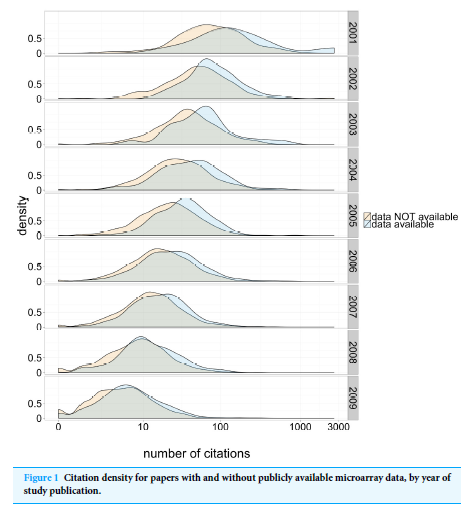
\includegraphics[height=\paperheight]{../images/peerj_piwowar_vision2013.PNG}
%            };
%        \end{tikzpicture}
%     \end{frame}
%}
%{ % all template changes are local to this group.
%    \setbeamertemplate{navigation symbols}{}
%    \begin{frame}[plain]
%        \begin{tikzpicture}[remember picture,overlay]
%            \node[at=(current page.center)] {
%                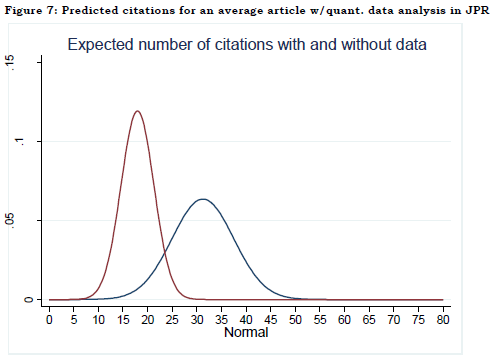
\includegraphics[width=\paperwidth]{../images/jpr.PNG}
%            };
%        \end{tikzpicture}
%     \end{frame}
%}
%
%\begin{frame}{The Case of Political Science}
%Exploit plausibly exogenous variation in data availability caused by the abrupt change in editorial policy at a top political science journal, \textit{The American Journal of Political Science} (\textit{AJPS}). 
%
%Rick Wilson became the editor on January 1, 2010:
%\begin{quote} ``If a manuscript is accepted for publication it will not be published unless the first footnote explicitly notes where the data used in the study can be obtained for purposes of replication and should note any sources that funded the research.''
%\end{quote}
%\end{frame}
%
%\begin{frame}{The Case of Political Science}
%The first issue Wilson edited was published in October 2010. After discussion with the board members in April of 2012, the policy was expanded to require posting data in the journal's public archive at \href{https://thedata.harvard.edu/dvn/dv/ajps}{Harvard's Dataverse} and Wilson strengthened his enforcement of this policy. This policy was printed in the July 2012 issue, and was enforced thereafter.
%\vspace{0.25in}
%
%There was no policy change at the other top political science journal, \textit{American Political Science Review}, (\textit{APSR}).
%\end{frame}
%
%\begin{frame}{The Case of Economics*}
%\begin{itemize}
%\item The Journal of Money, Credit, and Banking Project \href{http://www.jstor.org/stable/3132121}{(Dewald, Thursby, Anderson 1986)}
%\item Verifying the Solution from a Nonlinear Solver: A Case Study \href{http://www.jstor.org/stable/3132121}{(McCullough, Vinod 2003)}
%\item Ben Bernanke made the \textit{American Economic Review} policy mandatory in 2005.
%\item \textit{Quarterly Journal of Economics} didn't require data sharing until 2016.
%\end{itemize}
%\end{frame}
%
%{ % all template changes are local to this group.
%    \setbeamertemplate{navigation symbols}{}
%    \begin{frame}[plain]
%        \begin{tikzpicture}[remember picture,overlay]
%            \node[at=(current page.center)] {
%                
\includegraphics[width=\paperwidth]{../images/JMCB1.PNG}
%            };
%        \end{tikzpicture}
%     \end{frame}
%}
%\section{Methods}
%\begin{frame}{Pre-Analysis Plan}
%
%\begin{itemize}
%\item Short pre-analysis plan before data collection.
%\item Available at \url{https://osf.io/qxpr6/}
%\item Use 2SLS to estimate causal effect (LATE)
%\begin{itemize}
%\item \href{http://www.tandfonline.com/doi/abs/10.1080/01621459.1996.10476902}{Angrist, Imbens, Ruben (1993)}
%\item  \href{http://www.nber.org/papers/t0118}{Angrist, Imbens (1994)}
%\end{itemize} 
%\end{itemize}
%\end{frame}
%
%\begin{frame}{2SLS in 60 Seconds or Less}
%
%$$Y_i=\alpha + \beta \cdot X_i+u_i$$
%Problem: X of interest is endogenous. (Omitted variable bias--some unobservable is correlated with Y and X of interest.)
%
%\vspace{0.25in}
%Solution: Find an instrument. 
%$$corr(Z,u)=0$$
%$$corr(Z,X)\neq 0$$
%
%Biased, but consistent. (Get large N!)
%\end{frame}
%
%\begin{frame}{2SLS in More Detail}
%Implementation: 
%\begin{enumerate}
%\item Predict X with Z. (First Stage)
%\item Regress Y on predicted X's. (Second Stage)
%\item Adjust standard errors.
%\end{enumerate}
%Assumptions:
%\begin{itemize}
%\item Relevance. (Strong first stage, $corr(Z,X)\neq 0; F>10$)
%\item Exclusion Restriction.  ($corr(Z,u)=0$; Instrument only effects outcome through included X's.)
%\end{itemize}
%\end{frame}
%
%\begin{frame}{2SLS Examples}
%\begin{itemize}
%\item Best: Randomized Trial, incomplete adoption, use treatment assignment as instrument for treatment, get TOT and ITT. (Wald Estimator)
%\item Vietnam draft lottery predicts service, get unbiased effect of service on earnings.
%\item Quarter of Birth as instrument for schooling, get effect of schooling on earnings (with no ability bias).
%\item Settler mortality as instrument for institutions, get effect of institutions on GDP.
%\item Rainfall shocks predict GDP, get effect of GDP on civil conflict.
%\end{itemize}
%\end{frame}
%
%\begin{frame}{Our Estimation Strategy}
%\begin{align}\label{firststage} 
%availability_i &= \alpha_1 +\beta_1 AJPS_i + \beta_2 Post2010_i + \beta_3 Post2012_i \\ \notag
%& + {\color{red} \beta_4 AJPS*Post2010_i + \beta_5 AJPS*Post2012_i } \\
%& + g_1(Time) + h_1(Year) +\nu_i \notag
%\end{align}
%
%\begin{align}
%citations_i &=\alpha_2 +\eta_1 AJPS_i + \eta_2 Post2010_i+ \eta_3 Post2012_i \\ 
%& + \eta_4 \hat{availability_i}+g_2(Time) + h_2(Year) +u_i \notag
%\end{align}
%
%\end{frame}
%\begin{frame}{Summary Statistics}
%\begin{itemize}
%\item Citations highly concentrated.
%\item Citations increase over time.
%\item Citations affected by journal policy.
%\end{itemize}
%\end{frame}
%
%{ % all template changes are local to this group.
%    \setbeamertemplate{navigation symbols}{}
%    \begin{frame}[plain]
%        \begin{tikzpicture}[remember picture,overlay]
%            \node[at=(current page.center)] {
%                \includegraphics[width=\paperwidth]{../output/cite_histo.eps}
%
%            };
%        \end{tikzpicture}
%     \end{frame}
%     
%     \begin{frame}[plain]
%        \begin{tikzpicture}[remember picture,overlay]
%            \node[at=(current page.center)] {
%                \includegraphics[width=\paperwidth]{../output/cite_time.eps}
%
%            };
%        \end{tikzpicture}
%     \end{frame}
%    
%    \begin{frame}[plain]
%        \begin{tikzpicture}[remember picture,overlay]
%            \node[at=(current page.center)] {
%                \includegraphics[width=\paperwidth]{../output/avail_time.eps}
%            };
%        \end{tikzpicture}
%     \end{frame}
%}


\section{Results: OLS}
\begin{frame}
\begin{itemize}
\item Naive OLS results
\item First stage
\item 2SLS
\item Exclusion Restriction
\end{itemize}
\end{frame}

%\begin{frame}{}
%\scalebox{0.65}{\input{../output/both_naive.tex}}
%\end{frame}

\subsection{Naive OLS}
%%%%%%%%%%%%%%%%%%%%%%%%%%%%%%%%%%%%%%%%%%%%%%%
%%%NAIVE OLS
%%%%%%%%%%%%%%%%%%%%%%%%%%%%%%%%%%%%%%%%%%%%%%%
\begin{frame}{Naive OLS}

Full print:

Data and code. Months.

Data and code. FE.

Data. Months.

Data. FE.
\end{frame}

\begin{frame}{}
\scalebox{0.5}{\input{../output/both_naive_yn_months.tex}}
\end{frame}

\begin{frame}{}
\scalebox{0.5}{\input{../output/both_naive_yn_FE.tex}}
\end{frame}

\begin{frame}{}
\scalebox{0.5}{\input{../output/both_naive_data_months.tex}}
\end{frame}

\begin{frame}{}
\scalebox{0.5}{\input{../output/both_naive_data_FE.tex}}
\end{frame}

\begin{frame}{Naive OLS}
Simple Print:

Data and code. Months.

Data and code. FE.

Data. Months.

Data. FE.
\end{frame}

\begin{frame}{}
\scalebox{0.65}{\input{../output/both_naive-simp_yn_months.tex}}
\end{frame}

\begin{frame}{}
\scalebox{0.65}{\input{../output/both_naive-simp_yn_FE.tex}}
\end{frame}

\begin{frame}{}
\scalebox{0.65}{\input{../output/both_naive-simp_data_months.tex}}
\end{frame}

\begin{frame}{}
\scalebox{0.65}{\input{../output/both_naive-simp_data_FE.tex}}
\end{frame}

\subsection{Naive OLS Log}
%%%%%%%%%%%%%%%%%%%%%%%%%%%%%%%%%%%%%%%%%%%%%%%
%%%NAIVE OLS LOG
%%%%%%%%%%%%%%%%%%%%%%%%%%%%%%%%%%%%%%%%%%%%%%%
\begin{frame}{Naive OLS Log}
Full print:

Data and code. Months.

Data and code. FE.

Data. Months.

Data. FE.
\end{frame}

\begin{frame}{}
\scalebox{0.5}{\input{../output/both_naiveln_yn_months.tex}}
\end{frame}

\begin{frame}{}
\scalebox{0.5}{\input{../output/both_naiveln_yn_FE.tex}}
\end{frame}

\begin{frame}{}
\scalebox{0.5}{\input{../output/both_naiveln_data_months.tex}}
\end{frame}

\begin{frame}{}
\scalebox{0.5}{\input{../output/both_naiveln_data_FE.tex}}
\end{frame}

\begin{frame}{Naive OLS Log}
Simple Print:

Data and code. Months.

Data and code. FE.

Data. Months.

Data. FE.
\end{frame}

\begin{frame}{}
\scalebox{0.65}{\input{../output/both_naiveln-simp_yn_months.tex}}
\end{frame}

\begin{frame}{}
\scalebox{0.65}{\input{../output/both_naiveln-simp_yn_FE.tex}}
\end{frame}

\begin{frame}{}
\scalebox{0.65}{\input{../output/both_naiveln-simp_data_months.tex}}
\end{frame}

\begin{frame}{}
\scalebox{0.65}{\input{../output/both_naiveln-simp_data_FE.tex}}
\end{frame}

%%%%%%%%%%%%%%%%%%%%%%%%%%%%%%%%%%%%%%%%%%%%%%
\subsection{First Stage}
%% FIRST STAGE
%%%%%%%%%%%%%%%%%%%%%%%%%%%%%%%%%%%%%%%%%%%%

\begin{frame}{First Stage}
Full Print:

Data and code. Months.

Data and code. FE.

Data. Months.

Data. FE.
\end{frame}


\begin{frame}{}
\scalebox{0.5}{\input{../output/both_first_yn_months.tex}}
\end{frame}

\begin{frame}{}
\scalebox{0.5}{\input{../output/both_first_yn_FE.tex}}
\end{frame}

\begin{frame}{}
\scalebox{0.5}{\input{../output/both_first_data_months.tex}}
\end{frame}

\begin{frame}{}
\scalebox{0.5}{\input{../output/both_first_data_FE.tex}}
\end{frame}



\section{2SLS}
\subsection{2SLS Level}
%%%%%%%%%%%%%%%%%%%%%%%%%%%%%%%%%%%%%%%%%
%%2SLS LEVEL
%%%%%%%%%%%%%%%%%%%%%%%%%%%%%%%%%%%%%%%%
\begin{frame}{2SLS Level}
Full Print:

Data and code. Months.

Data and code. FE.

Data. Months.

Data. FE.
\end{frame}

\begin{frame}{}
\scalebox{0.45}{\input{../output/both_ivreg_yn_months.tex}}
\end{frame}

\begin{frame}{}
\scalebox{0.45}{\input{../output/both_ivreg_yn_FE.tex}}
\end{frame}

\begin{frame}{}
\scalebox{0.45}{\input{../output/both_ivreg_data_months.tex}}
\end{frame}

\begin{frame}{}
\scalebox{0.45}{\input{../output/both_ivreg_data_FE.tex}}
\end{frame}

\begin{frame}{2SLS Level}
Simple Print:

Data and code. Months.

Data and code. FE.

Data. Months.

Data. FE.
\end{frame}
\begin{frame}{}
\scalebox{0.6}{\input{../output/both_ivreg-simp_yn_months.tex}}
\end{frame}

\begin{frame}{}
\scalebox{0.6}{\input{../output/both_ivreg-simp_yn_FE.tex}}
\end{frame}

\begin{frame}{}
\scalebox{0.6}{\input{../output/both_ivreg-simp_data_months.tex}}
\end{frame}

\begin{frame}{}
\scalebox{0.6}{\input{../output/both_ivreg-simp_data_FE.tex}}
\end{frame}

\subsection{2SLS Log}
%%%%%%%%%%%%%%%%%%%%%%%%%%%%%%%%%%%%%%%%%
%%2SLS LOG
%%%%%%%%%%%%%%%%%%%%%%%%%%%%%%%%%%%%%%%%
\begin{frame}{2SLS Log}
Full Print:

Data and code. Months.

Data and code. FE.

Data. Months.

Data. FE.
\end{frame}

\begin{frame}{}
\scalebox{0.45}{\input{../output/both_ivregln_yn_months.tex}}
\end{frame}

\begin{frame}{}
\scalebox{0.45}{\input{../output/both_ivregln_yn_FE.tex}}
\end{frame}

\begin{frame}{}
\scalebox{0.45}{\input{../output/both_ivregln_data_months.tex}}
\end{frame}

\begin{frame}{}
\scalebox{0.45}{\input{../output/both_ivregln_data_FE.tex}}
\end{frame}

\begin{frame}{2SLS Log}
Simple Print:

Data and code. Months.

Data and code. FE.

Data. Months.

Data. FE.
\end{frame}

\begin{frame}{}
\scalebox{0.6}{\input{../output/both_ivregln-simp_yn_months.tex}}
\end{frame}

\begin{frame}{}
\scalebox{0.6}{\input{../output/both_ivregln-simp_yn_FE.tex}}
\end{frame}

\begin{frame}{}
\scalebox{0.6}{\input{../output/both_ivregln-simp_data_months.tex}}
\end{frame}

\begin{frame}{}
\scalebox{0.6}{\input{../output/both_ivregln-simp_data_FE.tex}}
\end{frame}

%\begin{frame}{Citation Data}
%Citations are interesting data in and of themselves.
%\begin{itemize}
%\item Multiple sources
%\item Not open
%\item Initiative to change that: \href{http://i4oc.org}{I4OC}
%\end{itemize}
%Results robust to source of citation data
%\end{frame}
%
%{ % all template changes are local to this group.
%    \setbeamertemplate{navigation symbols}{}
%    \begin{frame}[plain]
%        \begin{tikzpicture}[remember picture,overlay]
%            \node[at=(current page.center)] {
%                \includegraphics[width=\paperwidth]{../output/citationcomparison.eps}
%            };
%        \end{tikzpicture}
%     \end{frame}
%}
%
%{ % all template changes are local to this group.
%    \setbeamertemplate{navigation symbols}{}
%    \begin{frame}[plain]
%        \begin{tikzpicture}[remember picture,overlay]
%            \node[at=(current page.center)] {
%                \includegraphics[width=\paperwidth]{../output/topicXjournalXpost2010.eps}
%            };
%        \end{tikzpicture}
%     \end{frame}
%}
%
%
%{ % all template changes are local to this group.
%    \setbeamertemplate{navigation symbols}{}
%    \begin{frame}[plain]
%        \begin{tikzpicture}[remember picture,overlay]
%            \node[at=(current page.center)] {
%                \includegraphics[width=\paperwidth]{../output/topicXjournalXpost2012.eps}
%            };
%        \end{tikzpicture}
%     \end{frame}
%}
%
%{ % all template changes are local to this group.
%    \setbeamertemplate{navigation symbols}{}
%    \begin{frame}[plain]
%        \begin{tikzpicture}[remember picture,overlay]
%            \node[at=(current page.center)] {
%                \includegraphics[width=\paperwidth]{../output/typeXjournalXpost2010.eps}
%            };
%        \end{tikzpicture}
%     \end{frame}
%}
%
%{ % all template changes are local to this group.
%    \setbeamertemplate{navigation symbols}{}
%    \begin{frame}[plain]
%        \begin{tikzpicture}[remember picture,overlay]
%            \node[at=(current page.center)] {
%                \includegraphics[width=\paperwidth]{../output/typeXjournalXpost2012.eps}
%            };
%        \end{tikzpicture}
%     \end{frame}
%}
%
%{ % all template changes are local to this group.
%    \setbeamertemplate{navigation symbols}{}
%    \begin{frame}[plain]
%        \begin{tikzpicture}[remember picture,overlay]
%            \node[at=(current page.center)] {
%                \includegraphics[width=\paperwidth]{../output/rankXjournalXpost2010.eps}
%            };
%        \end{tikzpicture}
%     \end{frame}
%}
%
%{ % all template changes are local to this group.
%    \setbeamertemplate{navigation symbols}{}
%    \begin{frame}[plain]
%        \begin{tikzpicture}[remember picture,overlay]
%            \node[at=(current page.center)] {
%                \includegraphics[width=\paperwidth]{../output/rankXjournalXpost2012.eps}
%            };
%        \end{tikzpicture}
%     \end{frame}
%}

\section{Robustness}
\subsection{Exclusion Restriction}
%%%%%%%%%%%%%%%%%%%%%%%%%%%%%%%%%%%%%%%%%
%%Exclusion Restriction
%%%%%%%%%%%%%%%%%%%%%%%%%%%%%%%%%%%%%%%%
\begin{frame}{Exclusion Restriction}
Simple Print:

Data and code. Months.

Data and code. FE.

Data. Months.

Data. FE.
\end{frame}
\begin{frame}{}
\scalebox{0.61}{\input{../output/both_exclusion_yn_months.tex}}
\end{frame}
\begin{frame}{}
\scalebox{0.61}{\input{../output/both_exclusion_yn_FE.tex}}
\end{frame}
\begin{frame}{}
\scalebox{0.61}{\input{../output/both_exclusion_data_months.tex}}
\end{frame}
\begin{frame}{}
\scalebox{0.61}{\input{../output/both_exclusion_data_FE.tex}}
\end{frame}

\subsection{Partial/Stated Availability-OLS}
%%%%%%%%%%%%%%%%%%%%%%%%%%%%%%%%%%%%%%%%%
%%Partial/Stated OLS
%%%%%%%%%%%%%%%%%%%%%%%%%%%%%%%%%%%%%%%%
\begin{frame}{Naive OLS-Partial/Stated Availability}
Simple Print:

Stated Full. Months.

Stated Full. FE.

Stated Partial. Months.

Stated Partial. FE.
\end{frame}

\begin{frame}{}
\scalebox{0.65}{\input{../output/both_naive-simp_state_full_months.tex}}
\end{frame}

\begin{frame}{}
\scalebox{0.65}{\input{../output/both_naive-simp_state_full_FE.tex}}
\end{frame}

\begin{frame}{}
\scalebox{0.65}{\input{../output/both_naive-simp_state_part_months.tex}}
\end{frame}

\begin{frame}{}
\scalebox{0.65}{\input{../output/both_naive-simp_state_part_FE.tex}}
\end{frame}

%%%%%%%%%%%%%%%%%%%%%%%%%%%%%%%%%%%%%%%%%
%%Partial/Stated Log
%%%%%%%%%%%%%%%%%%%%%%%%%%%%%%%%%%%%%%%%
\begin{frame}{Naive OLS Log-Partial/Stated Availability}
Simple Print:

Stated Full. Months.

Stated Full. FE.

Stated Partial. Months.

Stated Partial. FE.
\end{frame}

\begin{frame}{}
\scalebox{0.65}{\input{../output/both_naiveln-simp_state_full_months.tex}}
\end{frame}

\begin{frame}{}
\scalebox{0.65}{\input{../output/both_naiveln-simp_state_full_FE.tex}}
\end{frame}

\begin{frame}{}
\scalebox{0.65}{\input{../output/both_naiveln-simp_state_part_months.tex}}
\end{frame}

\begin{frame}{}
\scalebox{0.65}{\input{../output/both_naiveln-simp_state_part_FE.tex}}
\end{frame}



%%%%%%%%%%%%%%%%%%%%%%%%%%%%%%%%%%%%%%%%%%%%%%
\subsection{Partial/Stated:First Stage}
%% PARTIAL/STATED-FIRST STAGE
%%%%%%%%%%%%%%%%%%%%%%%%%%%%%%%%%%%%%%%%%%%%

\begin{frame}{Partial/Stated Availability-First Stage}
Full Print:

State Full. Months.

State Full. FE.

State Part. Months.

State Part. FE.
\end{frame}


\begin{frame}{}
\scalebox{0.5}{\input{../output/both_first_state_full_months.tex}}
\end{frame}

\begin{frame}{}
\scalebox{0.5}{\input{../output/both_first_state_full_FE.tex}}
\end{frame}

\begin{frame}{}
\scalebox{0.5}{\input{../output/both_first_state_part_months.tex}}
\end{frame}

\begin{frame}{}
\scalebox{0.5}{\input{../output/both_first_state_part_FE.tex}}
\end{frame}


\subsection{Partial/Stated Availability-2SLS}
%%%%%%%%%%%%%%%%%%%%%%%%%%%%%%%%%%%%%%%%%
%%2SLS LEVEL-Partial/Stated
%%%%%%%%%%%%%%%%%%%%%%%%%%%%%%%%%%%%%%%%
\begin{frame}{2SLS Level-Partial/Stated}
Simple Print:

State Full. Months.

State Full. FE.

State Part. Months.

State Part. FE.
\end{frame}
\begin{frame}{}
\scalebox{0.6}{\input{../output/both_ivreg-simp_state_full_months.tex}}
\end{frame}

\begin{frame}{}
\scalebox{0.6}{\input{../output/both_ivreg-simp_state_full_FE.tex}}
\end{frame}

\begin{frame}{}
\scalebox{0.6}{\input{../output/both_ivreg-simp_state_part_months.tex}}
\end{frame}

\begin{frame}{}
\scalebox{0.6}{\input{../output/both_ivreg-simp_state_part_FE.tex}}
\end{frame}

%%%%%%%%%%%%%%%%%%%%%%%%%%%%%%%%%%%%%%%%%
%%2SLS LOG-Partial/Stated
%%%%%%%%%%%%%%%%%%%%%%%%%%%%%%%%%%%%%%%%
\begin{frame}{2SLS Log-Partial/Stated}
Simple Print:

State Full. Months.

State Full. FE.

State Part. Months.

State Part. FE.
\end{frame}

\begin{frame}{}
\scalebox{0.6}{\input{../output/both_ivregln-simp_state_full_months.tex}}
\end{frame}

\begin{frame}{}
\scalebox{0.6}{\input{../output/both_ivregln-simp_state_full_FE.tex}}
\end{frame}

\begin{frame}{}
\scalebox{0.6}{\input{../output/both_ivregln-simp_state_part_months.tex}}
\end{frame}

\begin{frame}{}
\scalebox{0.6}{\input{../output/both_ivregln-simp_state_part_FE.tex}}
\end{frame}

%%%%%%%%%%%%%%%%%%%%%%%%%%%%%%%%%%%%%%%%%%
\subsection{WoK Alternate Citation Measure}
\begin{frame}{Naive OLS-WoK Citations}
Simple Print:

Data and code. Months.

Data and code. FE.

Data. Months.

Data. FE.
\end{frame}

\begin{frame}{}
\scalebox{0.3}{\input{../output/both_naivewok-simp_yn_months.tex}}
\end{frame}

\begin{frame}{}
\scalebox{0.3}{\input{../output/both_naivewok-simp_yn_FE.tex}}
\end{frame}

\begin{frame}{}
\scalebox{0.3}{\input{../output/both_naivewok-simp_data_months.tex}}
\end{frame}

\begin{frame}{}
\scalebox{0.3}{\input{../output/both_naivewok-simp_data_FE.tex}}
\end{frame}
%%%%%%%%%%%%%%%%%%%%%%%%%%%%%%%%

\begin{frame}{2SLS WoK Citations}
Simple Print:

Data and code. Months.

Data and code. FE.

Data. Months.

Data. FE.
\end{frame}

\begin{frame}{}
\scalebox{0.3}{\input{../output/both_ivregwok-simp_yn_months.tex}}
\end{frame}

\begin{frame}{}
\scalebox{0.3}{\input{../output/both_ivregwok-simp_yn_FE.tex}}
\end{frame}

\begin{frame}{}
\scalebox{0.3}{\input{../output/both_ivregwok-simp_data_months.tex}}
\end{frame}

\begin{frame}{}
\scalebox{0.3}{\input{../output/both_ivregwok-simp_data_FE.tex}}
\end{frame}



%\section{Conclusion}
%
%\begin{frame}{Preliminary Conclusions}
%
%  % Keep the summary *very short*.
%  \begin{itemize}
%  \item
%    Top political science papers with public data are cited more.
%  \item
%    Some suggestive, not strong, evidence of causality.
%  \item
%    Journal policy does not appear to have changed submissions.
%    \begin{itemize}
%    \item IV identification strategy OK.
%    \end{itemize}
%  \end{itemize}
%\end{frame}
%
%\begin{frame}{Future}
%	\begin{itemize}
%	%\item Data quality checks.
%	\item Economics: AER \& QJE 2001-2009
%	\item Collaborate with Don Moore \& Andrew Rose
%	\begin{itemize}
%	\item Expand journals (19 with policy changes)
%	\item Narrow data collection
%	\end{itemize}
%	\end{itemize}
%\end{frame}

\end{document}


